% Preparation guide for the supervisor's review of the TM-RIS receiver project.
% Build: pdflatex supervisor_guide.tex (twice). Figures are read from ../paper/ieee/.
\documentclass[11pt,a4paper]{article}
\usepackage[T1]{fontenc}
\usepackage{lmodern,microtype}
\usepackage[margin=2.2cm]{geometry}
\usepackage{amsmath,amssymb,bm}
\usepackage{graphicx,booktabs,tabularx,longtable,enumitem,xcolor}
\usepackage[most]{tcolorbox}
\usepackage[hidelinks]{hyperref}
\usepackage{fancyhdr,titlesec}
\graphicspath{{../paper/ieee/}}
\definecolor{cA}{HTML}{2a78d6}
\definecolor{cB}{HTML}{eb6834}
\definecolor{cG}{HTML}{1baf7a}
\definecolor{mut}{HTML}{52514e}
\setlist{itemsep=1pt,topsep=3pt}
\titleformat{\section}{\Large\bfseries\color{cA}}{\thesection}{0.6em}{}
\titleformat{\subsection}{\large\bfseries}{\thesubsection}{0.6em}{}
\pagestyle{fancy}\fancyhf{}\rhead{\small TM-RIS receiver: preparation guide}\cfoot{\thepage}
\renewcommand{\headrulewidth}{0.3pt}
\newtcolorbox{keybox}[1][]{colback=cA!6,colframe=cA,boxrule=0.6pt,arc=2pt,left=6pt,right=6pt,top=4pt,bottom=4pt,#1}
\newtcolorbox{warnbox}[1][]{colback=cB!7,colframe=cB,boxrule=0.6pt,arc=2pt,left=6pt,right=6pt,top=4pt,bottom=4pt,#1}
\newcommand{\say}[1]{\begin{keybox}\textbf{Say:} \emph{#1}\end{keybox}}
\newcounter{qn}
\newcommand{\Q}[1]{\stepcounter{qn}\par\medskip\noindent\textbf{Q\theqn.\ #1}\par\nopagebreak\noindent}
\newcommand{\T}{\mathsf T}

\begin{document}

\begin{titlepage}
\centering
\vspace*{3cm}
{\Huge\bfseries\color{cA} Receiver for Time-Modulated RIS\\[0.3em] in OFDM with Non-Ideal Elements\par}
\vspace{1cm}
{\Large Preparation guide for the supervisor's review\par}
\vspace{1.5cm}
{\large Architecture, theory, every figure and table, the repository,\\ the negative results, and the questions to expect, with answers\par}
\vfill
{\normalsize Project repository: \texttt{tm\_ris\_ofdm/}\quad Paper: \texttt{paper/ieee/tm\_ris\_receiver\_ieee.pdf} (11 pages)\par}
\vspace{0.5cm}
{\normalsize 28 October 2026\par}
\end{titlepage}

\tableofcontents
\newpage

%=====================================================================
\section{The project in one paragraph}
A \textbf{time-modulated RIS (TM-RIS)} switches each element between two states several times inside every OFDM symbol.
Switching inside a symbol spreads each transmitted subcarrier onto many received subcarriers, so the channel stops being
diagonal. Earlier TM-RIS papers use this deliberately, for security or to steer energy to harmonic frequencies. They
assume ideal elements (a perfect $\pm1$ switch) and treat the coupling as interference for the intended user.

Real varactor elements are \textbf{frequency-dependent and not ideal}. Iudice et al.\ (Sept.\ 2026) built the physically
correct model of this channel. They assumed the channel is known and listed \textbf{equalization as future work}. Nobody
had built the receiver: estimating this channel from pilots and then equalizing it.

\begin{keybox}
\textbf{Our contribution is that receiver.} It rests on one exact identity (Proposition~1): the coupling splits into a
part the receiver already knows (the switching \emph{timing}) and a part it must learn (the propagation together with the
element response). Because of that split, the receiver never needs a model of the element.
\end{keybox}

%=====================================================================
\section{Background, in the order your supervisor will think about it}
\begin{enumerate}
\item \textbf{OFDM.} With a cyclic prefix and a time-invariant channel, every subcarrier sees one complex gain. The channel
matrix $\bm H$ is diagonal and a one-tap equalizer suffices.
\item \textbf{Static RIS.} A passive surface that reflects with a chosen phase. The channel is still time-invariant, so
$\bm H$ stays diagonal.
\item \textbf{Time-modulated RIS.} Each element follows a pattern $s_q[k]\in\{1,2\}$ over $K$ slots per symbol. Here
$K=8$ and the duty cycle is $D=0.75$: 6 slots in state~1 and 2 in state~2. The reflection is periodic in time, i.e.\
multiplication by a periodic waveform. In frequency that is convolution with its Fourier series, so subcarrier $m$ leaks
onto subcarrier $m+h$ with weight equal to the $h$-th Fourier coefficient. \textbf{$\bm H$ becomes a full $M\times M$
matrix.}
\item \textbf{The element is not ideal.} In state $s$ the element reflects with a single-resonance response
\[ \Gamma_s(f) = -1 + \frac{2\xi_r}{j2\pi(f-f_0)+\xi_r+\xi_i}. \]
This is the published OpenRIS cell (Iudice et al., Table~I): resonances at 3.471 and 3.710\,GHz, $\xi_r/2\pi = 97.5$ /
128.4\,MHz, $\xi_i/2\pi = 8.9$ / 9.0\,MHz, common phase $-10.7^\circ$. The carrier is $f_c=3.594$\,GHz (5G band n78,
30\,kHz spacing). Across the 100\,MHz channel the phase of each state drifts by about 47--49$^\circ$, and $\Gamma_1\neq
-\Gamma_2$. A $\pm1$ model is wrong in two ways: the phase relation between the two states, and the frequency dependence.
\item \textbf{The ground truth} is Iudice's input--output relation (eq.~(io) in the paper):
\[ H(\bar m, m) = \sum_q a^{\rm d}_q(f_{\bar m})\; b_q^{[\bar m-m]}(f_m)\; a^{\rm s}_q(f_m), \]
where $a^{\rm s}$ is the base-station-to-element channel, $a^{\rm d}$ the element-to-user channel, and $b^{[h]}$ the
$h$-th Fourier coefficient of the switched element response. Our implementation matches an independent time-domain
simulation (filter, gate, FFT) to a median error of 0.27\%.
\end{enumerate}

%=====================================================================
\section{The core idea: Proposition 1 (know this cold)}
\paragraph{Statement.}
\[ b_q^{[h]}(f) = \sum_s t_{q,s}[h]\,\Gamma_s(f), \qquad
t_{q,s}[h] = \frac{e^{-j\pi h/K}}{K}\,\mathrm{sinc}\!\left(\frac hK\right) \sum_{k:\,s_q[k]=s} e^{-j2\pi hk/K}. \]
Therefore
\[ \bm H = \sum_q\sum_s \bm T_{q,s}\circ\big(\bm a^{\rm d}_q\,\bm v_{q,s}^{\T}\big), \qquad
\bm v_{q,s} = \bm\Gamma_s\odot\bm a^{\rm s}_q. \]

\paragraph{Proof idea.} In slot $k$ the element applies $\Gamma$ of state $s_q[k]$, so its response is
$\sum_s\Gamma_s(f)\,\mathbb 1_s(t)$. The Fourier coefficient of a slot indicator is a sinc times a phase. The sum over the
slots in state $s$ depends only on $h=\bar m-m$, which gives a Toeplitz matrix $\bm T$.

\paragraph{What it means.}
\begin{itemize}
\item \textbf{The $\bm T$ matrices} depend only on the switching pattern (timing), which the network sets, so the receiver
knows them. They are Toeplitz.
\item \textbf{The element response $\Gamma_s$} appears only inside $\bm v_{q,s}$, multiplied together with the unknown
BS--RIS channel. The receiver estimates $\bm v$ as one unknown, so it \textbf{never needs $\Gamma$}. This is Corollary~1,
``no element model''.
\item \textbf{$\bm H$ itself is not Toeplitz}, because $\bm v$ depends on the input frequency. That is why Toeplitz-based
methods fail here.
\end{itemize}
\begin{warnbox}
\textbf{Honesty point.} The regrouping itself is elementary, and the paper credits it to Iudice's model. The novelty is
what it implies for building a receiver.
\end{warnbox}

\subsection{The other corollaries and propositions}
\begin{itemize}
\item \textbf{Cor.~2, one-tap ceiling.} For ideal elements the DC term is $2D-1$ and the total energy is 1 (Parseval). A
one-tap receiver captures $(2D-1)^2$ and sees the rest as interference, so its SIR is at most
$(2D-1)^2/(1-(2D-1)^2)$ $=$ \textbf{$-4.8$\,dB at $D=0.75$}. A conventional receiver can never work.
\item \textbf{Cor.~3, harmonic tail.} $|t[h]|\le|\mathrm{sinc}(h/K)|\sim 1/h$, so the energy beyond $\pm H$ decays like
$1/H$: 3.4\% at $H=12$, 1.0\% at 40, 0.32\% at 128. Any model truncated to 12 harmonics has an error floor of
\textbf{$-14.7$\,dB}, whatever its estimator. That is why CE-BEM fails.
\item \textbf{Cor.~4, fast products.} $(\bm T\circ(\bm a\bm b^{\T}))\bm x = \bm a\odot(\bm T(\bm b\odot\bm x))$, and $\bm T\bm z$
is a convolution. So \textbf{$\bm H\bm x$ costs $O(QM\log M)$ with FFTs}, and $\bm H$ never has to be formed.
\item \textbf{Prop.~2, offset = opposite delay.} If the switching runs $d$ slots late, each kernel becomes $\bm D\bm T\bm D^*$,
and $(\bm D\bm T\bm D^*)\circ(\bm a\bm b^{\T}) = \bm T\circ((\bm D\bm a)(\bm D^*\bm b)^{\T})$. A timing offset looks exactly
like delaying the user hop and advancing the BS hop. Consequence: a wrong offset can still fit the pilots, so plain
residual fitting is ambiguous.
\item \textbf{Prop.~3, physical timing.}
  \begin{itemize}
  \item If the RIS controller is locked to the signal arriving at the RIS, there is no effective offset.
  \item If it is locked to the BS clock, the offset is $d=-\tau_b K/T_u$: its distance to the BS, tens to hundreds of ns.
  \item Ignoring that offset costs 1.6 / 4.2\,bit/s/Hz at 20 / 30\,dB.
  \item Both identities are verified numerically to $7\cdot10^{-15}$.
  \end{itemize}
\end{itemize}

%=====================================================================
\section{Receiver architecture}
\begin{figure}[h]\centering
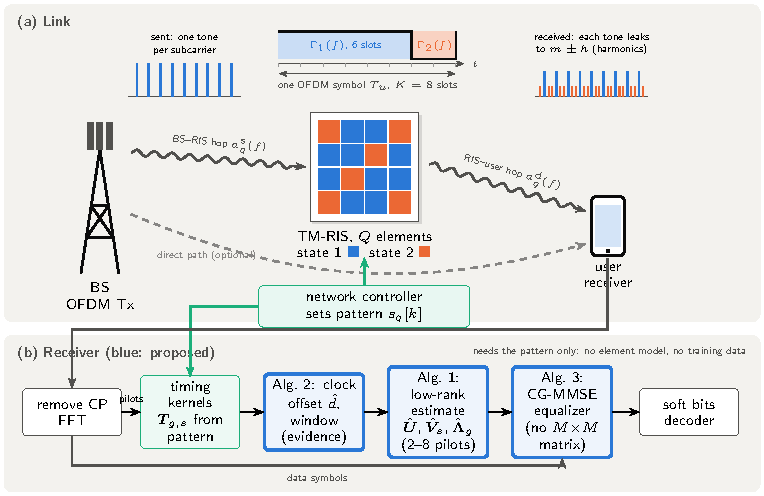
\includegraphics[width=\textwidth]{fig_system.pdf}
\caption*{\small Paper Fig.~1. (a) the link; (b) the receiver chain (blue: the proposed algorithms).}
\end{figure}

\subsection{How to read Fig.~1}
\textbf{Panel (a), the link.}
\begin{itemize}
\item \textbf{Left:} the base station sends OFDM; the inset shows one clean tone per subcarrier.
\item \textbf{Centre:} the TM-RIS, a $4\times4$ panel ($Q=16$ elements). Blue squares are elements in state~1, orange in
state~2, at one instant. The inset above shows the switching pattern over one OFDM symbol: $K=8$ slots, 6 in state~1
($\Gamma_1(f)$) and 2 in state~2 ($\Gamma_2(f)$).
\item \textbf{Wavy arrows:} the two hops, BS--RIS $a^{\rm s}_q(f)$ and RIS--user $a^{\rm d}_q(f)$. Dashed: an optional
direct path.
\item \textbf{Right:} the user. Its received-spectrum inset shows each tone leaking onto neighbouring tones $m\pm h$ (the
harmonics). That leakage is the non-diagonal $\bm H$.
\item \textbf{Bottom (green):} the network controller sets the pattern $s_q[k]$ and sends it both to the RIS and to the
receiver. That is assumption A1.
\end{itemize}
\textbf{Panel (b), the receiver chain.} Remove CP, FFT $\to$ timing kernels $\bm T_{g,s}$ computed from the pattern (green:
computed, not estimated) $\to$ Algorithm~2 $\to$ Algorithm~1 $\to$ Algorithm~3 $\to$ soft bits and decoder. The data
symbols bypass the estimator and go straight to the equalizer.
\say{The network knows the pattern, so the receiver computes the timing kernels and learns only the propagation and the
element response, never an element model and never the $M\times M$ matrix.}

\subsection{The low-rank model (eq.~(model))}
\textbf{Shared paths (A4).} On a compact surface all elements see the same physical paths and differ only by geometric
phases. So the stacked user-hop responses $[\bm a^{\rm d}_1\cdots\bm a^{\rm d}_Q]$ have rank at most the number of paths,
however large $Q$ is.

\textbf{Delay basis.} Each hop response is delay-limited to a window of length $\tau_{\max}$. We represent it in the first
$L$ \textbf{DPSS (Slepian) vectors}, the optimal basis for delay-limited responses; their eigenvalues serve as prior
variances. The element response $\Gamma_s$ is smooth (memory 13.8\,ns), so $\mathrm{diag}(\Gamma_s)\bm E'$ stays inside the
same DPSS span, with a state-specific coefficient matrix $\bm V_s$. Result:
\[ \bm H = \sum_g\sum_s \bm T_{g,s}\circ\big((\bm F\bm U)\,\bm\Lambda_g\,(\bm F\bm V_s)^{\T}\big). \]
\begin{itemize}
\item $\bm U$ and $\bm V_s$ are $L\times r$; $\bm\Lambda_g$ is $r\times r$, one for each of the $G$ distinct patterns.
\item The unknowns drop from $M^2$ (65{,}536 at $M=256$) to \textbf{$3Lr+Gr^2$}, which is 448 for $L=16$, $r=8$, $G=1$.
\item A direct path (not via the RIS) is a special case, because $\bm T_1+\bm T_2=\bm I$. It needs no change.
\end{itemize}

\subsection{Algorithm 1: timing-only estimation}
\begin{enumerate}
\item \textbf{Pilot regressors.} Precompute $\bm G_{g,s,p}=\bm T_{g,s}\,\mathrm{diag}(\bm s_p)\,\bm F$ by FFT.
\item \textbf{Initialization from a linear model.} Ignore the low-rank structure and estimate
$\bm H\approx\sum_s\bar{\bm T}_s\circ(\bm F\bm C_s\bm F^{\T})$ with an LMMSE, using prior $\bm\lambda\otimes\bm\lambda$ scaled
by moment matching (exact for $G=1$). Then take a rank-$r$ SVD of $[\hat{\bm C}_1\ \hat{\bm C}_2]$ to initialize $\bm U$,
$\bm V$, and $\bm\Lambda=\bm I$.
\item \textbf{ALS iterations.} Alternate LMMSE updates of $\bm\Lambda$, $\bm U$ and $[\bm V_1;\bm V_2]$. The model is linear
in each block when the others are fixed, and the square-root form of the LMMSE stays well-posed when prior variances are
tiny.
\end{enumerate}
\begin{itemize}
\item \textbf{Convergence:} non-convex. Initialized from the linear estimate, ALS converges in 1--2 iterations; random
starts end up 3--5$\times$ worse.
\item \textbf{Removed fallback:} the old ``keep the linear estimate if it fits better'' rule was an overfitting trap on
fresh channels (pre-registered test G3b), so it was taken out.
\end{itemize}
\textbf{Why 2 pilots are enough.} 448 unknowns against 512 observations looks barely determined. But the prior concentrates
each hop on about $M\Delta f\tau_{\max}+1$ dimensions. The measured effective degrees of freedom (trace of the LMMSE hat
matrix) are only 19--27 at 20\,dB. The linear stage sits 5--6\,dB above the Bayesian bound ($-26.4$ vs $-32.4$\,dB). That
gap comes from real channels not following the uniform-delay prior, not from a suboptimal estimator.

\subsection{Algorithm 2: offset and window by evidence}
\begin{itemize}
\item \textbf{The problem.} By Prop.~2 the pilot residual is almost flat in the offset $d$ (a wrong $d$ overfits through
shifted responses).
\item \textbf{The fix.} Use the \textbf{log-evidence} (marginal likelihood, type-II ML)
$\ \mathcal E = -\bm y^{\rm H}\bm C^{-1}\bm y - \log\det\bm C$, with $\bm C=\bm\Phi\bm P\bm\Phi^{\rm H}+\sigma^2\bm I$.
The log-det term penalizes improbable shifted responses. It is computed through a Cholesky factorization and the
Woodbury identity, one factorization of size $2L^2$ per candidate.
\item \textbf{Search.} For each window start $t_0\in\{-150,-75,0,75\}$\,ns: a 41-point grid over $d$, refined by a 14-step
golden-section search; take the joint maximum.
\item \textbf{Results:} within noise of known timing; 5--58$\times$ cheaper than residual search (3.2 vs 17.2\,s; 11.7 vs
674\,s on TDL-C); with a single pilot the residual overfits (worse by 1.49 / 2.83\,bit/s/Hz) while the evidence does not.
\end{itemize}

\subsection{Algorithm 3: CG-MMSE equalizer}
\begin{itemize}
\item \textbf{What it solves:} $(\hat{\bm H}^{\rm H}\hat{\bm H}+\sigma^2\bm I)\bm x=\hat{\bm H}^{\rm H}\bm y$ by conjugate
gradients. Each product uses the factors and batched FFTs, so the representation is exact (unlike the BEM approximation in
Hrycak et al.).
\item \textbf{Tolerance} $3\cdot10^{-3}$, chosen by a pre-registered sweep: at $10^{-2}$ the error rate is 1.15$\times$ the
dense solver's; at $3\cdot10^{-3}$ it is within 2\%, after 8--20 iterations.
\item \textbf{Measured speed.} At $M=3276$ the dense solver takes 2.5\,s per estimate, almost independent of how many
symbols are equalized; CG takes about 0.2\,s per symbol.
  \begin{itemize}
  \item \textbf{Break-even is about 12 symbols per estimate}, not the 140 that operation counting predicts, because dense
  LAPACK runs as level-3 BLAS.
  \item CG wins for the 6--15-symbol refresh blocks used at 30 and 120\,km/h; dense wins (3--9$\times$) for slow channels.
  \item CG's lasting advantage is \textbf{memory linear in $M$}: it handles $M=6552$ without the 687\,MB matrix.
  \item The old ``2.6$\times$ faster'' claim was withdrawn.
  \end{itemize}
\end{itemize}

%=====================================================================
\section{The figures in the paper, and how to read each one}
The paper has eight figures. Every multi-panel figure is made of separately drawn graphs, and each graph follows the format
of the base paper it compares with: Iudice et al.\ for the element and coupling figures, Tang et al.\ (CE-BEM) for the SNR
and pilot figures. \textbf{$\bigstar$ marks the most important.}

\subsection*{Fig.~1: system and receiver (illustrated diagram)}
Explained in Section~4.

\subsection*{Fig.~2: the OpenRIS element, in the format of Iudice et al.\ Figs.~2--4}
\begin{center}
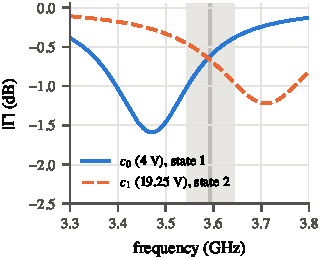
\includegraphics[width=0.32\textwidth]{fig_element_mag.pdf}\hfill
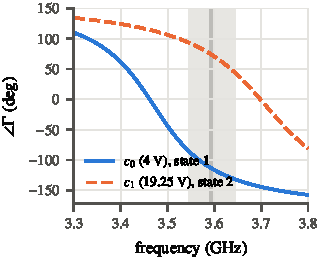
\includegraphics[width=0.32\textwidth]{fig_element_phase.pdf}\hfill
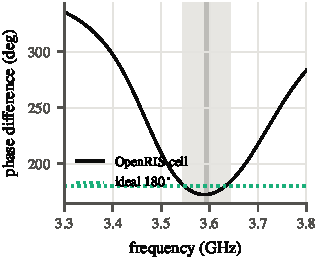
\includegraphics[width=0.32\textwidth]{fig_element_dphase.pdf}
\end{center}
Three graphs over 3.3--3.8\,GHz. The light band is the 100\,MHz channel; the dark strip is the 7.7\,MHz band of the
$M=256$ comparisons.
\begin{itemize}
\item \textbf{(a) Magnitude $|\Gamma|$ in dB.} Each state dips near its resonance (3.471 and 3.710\,GHz). In the channel
the two states differ by up to 0.57\,dB and the reflection loss is at most 1.01\,dB (Iudice: $\le0.75$\,dB, $<1.1$\,dB).
\item \textbf{(b) Phase $\angle\Gamma$.} Each state's phase drifts by 46.4$^\circ$ / 49.1$^\circ$ across the channel
(Iudice: 47$^\circ$ / 50$^\circ$).
\item \textbf{(c) Phase difference between the states}, against the ideal 180$^\circ$ line. It is $180^\circ\pm7.8^\circ$
across the channel (Iudice: $\pm6.5^\circ$). Over the 7.7\,MHz strip it is 172.2--172.5$^\circ$, i.e.\ a static
$\approx7.7^\circ$ error, not dispersion.
\end{itemize}
\say{The two states are not exact opposites and they drift with frequency; our single-pole model reproduces Iudice's
full-wave numbers to within about a degree and a fraction of a dB.}
\begin{warnbox}
Likely probe: \emph{why do your numbers differ slightly from Iudice's?} Iudice's figures come from full-wave simulation; we
use their fitted single-pole model with their Table~I parameters. The small differences ($\pm7.8^\circ$ vs $\pm6.5^\circ$,
0.57 vs 0.75\,dB) are the fit error of the single-pole model.
\end{warnbox}

\subsection*{Fig.~3: coupling-matrix structure, reproducing Iudice et al.\ Fig.~5}
\begin{center}
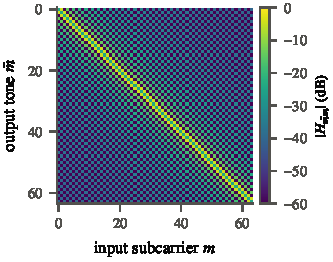
\includegraphics[width=0.32\textwidth]{fig_coupling_K2.pdf}\hfill
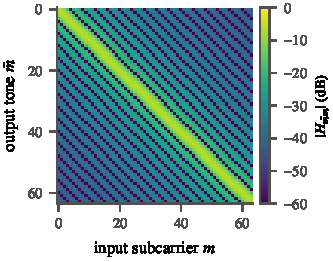
\includegraphics[width=0.32\textwidth]{fig_coupling_K8.pdf}\hfill
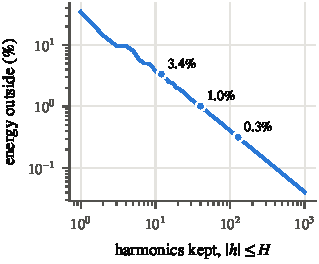
\includegraphics[width=0.32\textwidth]{fig_coupling_tail.pdf}
\end{center}
One element, ideal single-tap channels, $M=64$, OpenRIS cell, colour $|H_{\bar mm}|$ from 0 to $-60$\,dB (viridis, as in
Iudice).
\begin{itemize}
\item \textbf{(a) $K=2$, Iudice's setting.} Our implementation reproduces their Fig.~5: a bright main diagonal and a
\textbf{checkerboard} off the diagonal. With two equal slots the switching waveform is a square wave, whose even harmonics
vanish, so every second off-diagonal is dark.
\item \textbf{(b) $K=8$, $D=0.75$, our setting.} A broad bright band around the diagonal ($h=0,\pm1,\ldots$) and parallel
stripes that fade with distance from it (the harmonics). Dark lines recur every 4 diagonals: $t[h]=0$ when $h$ is a
multiple of 4 for this 6+2 pattern (the 2-slot block cancels, and the sinc is zero at multiples of 8).
\item \textbf{(c) Harmonic tail.} Fraction of coupling energy outside $|h|\le H$, log--log: falls as $1/H$; markers 3.4\%,
1.0\%, 0.32\% at $H=12$, 40, 128 (Corollary~3).
\end{itemize}
\say{(a) shows our code reproduces the published model; (b) shows the matrix our receiver must estimate is full, not
diagonal; (c) shows why any truncated-harmonic model has an error floor.}

\subsection*{$\bigstar$ Figs.~4 and 5: estimators versus SNR, in the format of Tang et al.\ (CE-BEM) Figs.~10--11}
\begin{center}
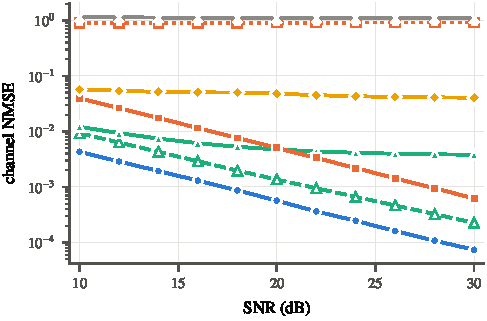
\includegraphics[width=0.48\textwidth]{fig_snr_phys30_nmse.pdf}\hfill
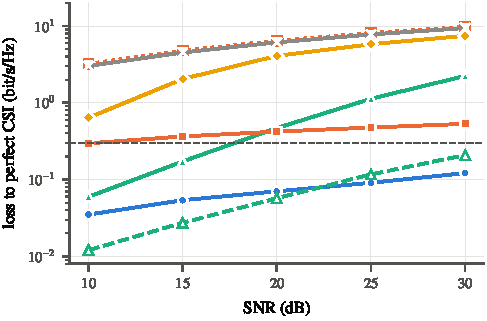
\includegraphics[width=0.48\textwidth]{fig_snr_phys30_loss.pdf}\\[2pt]
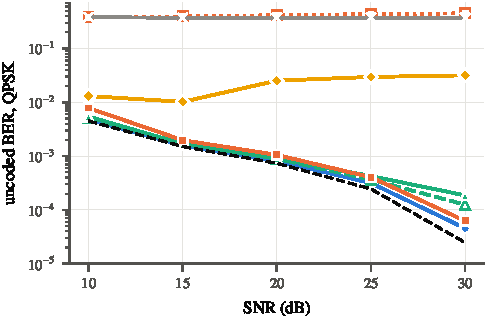
\includegraphics[width=0.48\textwidth]{fig_snr_phys30_ber4.pdf}\hfill
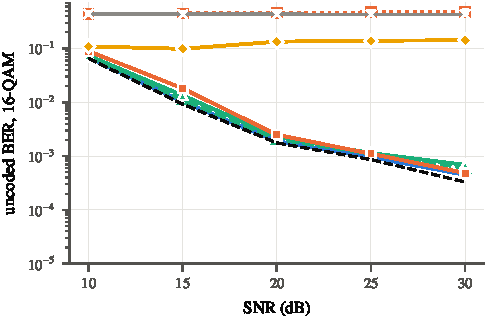
\includegraphics[width=0.48\textwidth]{fig_snr_phys30_ber16.pdf}\\[2pt]
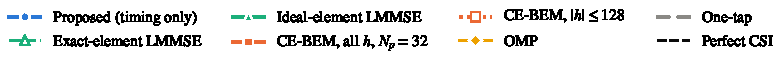
\includegraphics[width=0.85\textwidth]{fig_snr_legend.pdf}\\
{\small Fig.~4: shared-path channel, 2 pilots. Fig.~5 is the same four graphs on TDL-C (100\,ns) with 4 pilots.}
\end{center}
\textbf{Setup.} 10--30\,dB in 2\,dB steps, 30 channels per point, uncoded BER after unbiased MMSE for QPSK
($7.7\cdot10^5$ bits/point) and 16-QAM ($1.5\cdot10^6$). CE-BEM with all harmonics is given 32 pilots (16$\times$ ours on the
shared path, 8$\times$ on TDL-C). Points with zero errors are omitted.

\textbf{The curves:} ours (blue, filled circles); exact-element LMMSE (green dashed, open triangles: a genie reference given
the true $\Gamma$); ideal-element LMMSE (green solid: the literature's assumption); CE-BEM, all harmonics, 32 pilots (orange
solid); CE-BEM $|h|\le128$ at our pilots (orange dotted); OMP (yellow); one-tap (grey); perfect CSI (black dashed, BER only).

\paragraph{(a) Channel NMSE} (linear, log axis, as in Tang).
\begin{itemize}
\item Shared path: ours falls from $-23.7$ to $-41.3$\,dB, the lowest at every SNR. Exact-element runs about 3--5\,dB above
ours ($-20.3$ to $-36.5$). Ideal-element floors at $-24$\,dB (model-error floor). CE-BEM (32 pilots) improves from $-14$ to
$-32$\,dB. OMP floors near $-13$\,dB. One-tap and CE-BEM $|h|\le128$ sit near 0\,dB (no estimate).
\item TDL-C: ours $-18.8$ to $-32.6$\,dB, lowest from 16\,dB up; it begins to flatten above about 25\,dB (see the
high-SNR discussion below).
\end{itemize}
\paragraph{(b) Rate loss against perfect CSI} (log axis; dashed line 0.3\,bit/s/Hz). The graph to discuss.
\begin{center}\small
\begin{tabular}{lcc}
\toprule
Estimator (Fig.~4, shared path) & loss at 20\,dB & loss at 30\,dB \\
\midrule
Ours & 0.070 & 0.121\\
Exact-element LMMSE (genie) & 0.057 & 0.209\\
Ideal-element LMMSE & 0.469 & 2.24\\
CE-BEM, all $h$, 32 pilots & 0.421 & 0.532\\
OMP & 4.09 & 7.48\\
\bottomrule
\end{tabular}
\end{center}
\begin{itemize}
\item Shared path: ours stays between 0.035 and 0.121, below the 0.3 line throughout.
\item At low SNR the exact-element genie is slightly better than ours (by $\le0.03$ shared, $\le0.06$ TDL-C). The order
reverses at 22\,dB on these shared-path channels and 17\,dB on TDL-C (between 15 and 20\,dB on the earlier channel set).
Reason: a linear LMMSE with the right structure needs no nonlinear fit, which matters when noise dominates.
\item TDL-C: ours crosses 0.3 at 22\,dB and reaches 0.83 at 30\,dB; CE-BEM (32 pilots) 1.22 / 1.66; ideal-element 0.68 / 2.72.
\end{itemize}
\paragraph{(c), (d) Uncoded BER, QPSK and 16-QAM.} Ours tracks the perfect-CSI curve most closely among the practical
estimators. On the shared path it sits almost on top of it (within about $2\times$ up to 30\,dB); ideal-element bends away at
high SNR; OMP floors at $\sim3\cdot10^{-2}$ (QPSK) and $\sim10^{-1}$ (16-QAM).

\textbf{Key message:} the middle of the comparison is populated: a continuous ordering, not ``ours versus garbage''.
\begin{keybox}
\textbf{Why ours beats even the exact-element genie at high SNR:} it has \emph{fewer unknowns} (rank 8 against $L^2=256$
coefficients), so it removes more noise. Not because it knows more.
\end{keybox}

\paragraph{Why the graphs stop at 30 dB, and what happens above.} The same run (Step~11) also covered 35--40\,dB on a 5\,dB
grid; the text of the paper reports it:
\begin{itemize}
\item Shared path: ours keeps the lowest NMSE ($-48.4$\,dB at 40\,dB) and a loss of 0.26 at 40\,dB, against 0.46
(exact-element), 0.67 (CE-BEM, 32 pilots) and 5.4 (ideal-element).
\item TDL-C: every estimator approaches a floor. Ours loses 2.3 at 40\,dB, still the lowest rate loss (CE-BEM 2.46,
exact 3.0, ideal 5.96) and the lowest NMSE ($-34.5$ vs $-31.4$\,dB). But \textbf{from about 33\,dB CE-BEM with 8$\times$ our
pilots reaches the lower BER} (16-QAM at 40\,dB: $2.8\cdot10^{-4}$ vs ours $7.1\cdot10^{-4}$).
\end{itemize}
\begin{warnbox}
\textbf{The high-SNR floor, explained.} It is a model-error floor, not a failure of the method. Our estimator describes the
channel with a fixed number of parameters (rank 16, a finite delay window). TDL-C has many delay taps, so that description
is off by about $-34$\,dB. Below $\sim$25\,dB, noise is larger than this error and you do not see it; above, the error
dominates. Perfect CSI has no such error and keeps improving, so the gap opens. Every estimator has such a floor; the
ideal-element one floors much earlier, at about $-22$\,dB. Practical links mostly operate at 0--30\,dB, where we win on
every metric. More pilots or a higher rank should lower the floor (Fig.~7 shows about 3\,dB per doubling of pilots on the
shared path), but that has \emph{not} been tested on TDL-C at high SNR: say ``expected'', not ``shown''.
\end{warnbox}

\subsection*{$\bigstar\bigstar$ Fig.~6: loss against element non-ideality $\alpha$ (most important for a skeptical reader)}
\begin{center}
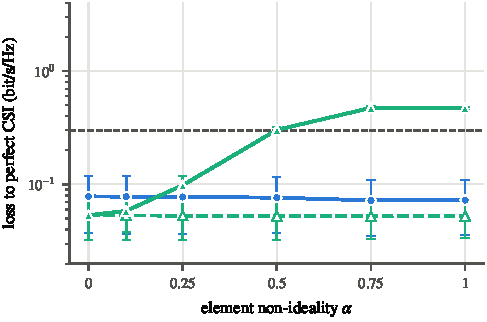
\includegraphics[width=0.48\textwidth]{fig_alpha_20dB.pdf}\hfill
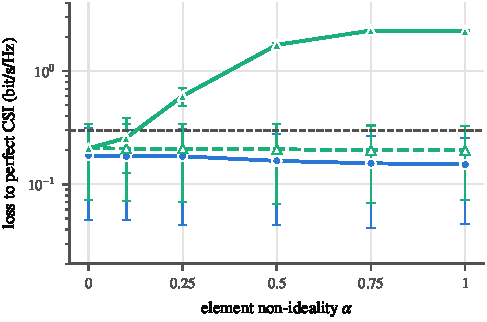
\includegraphics[width=0.48\textwidth]{fig_alpha_30dB.pdf}\\[2pt]

\includegraphics[width=0.7\textwidth]{fig_alpha_legend.pdf}
\end{center}

\paragraph{The question it answers.} Earlier TM-RIS papers assume each element is a perfect switch: state~1 reflects
with $+1$, state~2 with $-1$. The real OpenRIS cell does not: its two states are not exact opposites (a static
$\approx7.7^\circ$ phase error and a 0.57\,dB magnitude imbalance at the carrier). Fig.~6 asks: \emph{how much does each
receiver suffer as the element moves from the textbook switch to the real cell?}

\paragraph{What $\alpha$ is.} We cannot build an element ``halfway'' between ideal and real, but we do not need to. The
channel matrix is linear in the reflection coefficients (Proposition~1: $\Gamma_s$ appears once, as a factor), so blending
the coefficients blends the channels:
\[
\bm H_\alpha=(1-\alpha)\,\bm H_{\rm ideal}+\alpha\,\bm H_{\rm OpenRIS},\qquad
\Gamma_{s,\alpha}(f)=(1-\alpha)(\pm1)+\alpha\,\Gamma_{s,\rm OpenRIS}(f).
\]
$\alpha=0$: perfect $\pm1$ switch (the assumption of the literature). $\alpha=1$: the real cell. In between: a
progressively less ideal element. Everything else (propagation, pilots, noise) is identical along the axis; the same
30 channels are reused at every $\alpha$, so the curves differ only because of the element.

\paragraph{How to read the axes.} x-axis: $\alpha$. y-axis (log scale): \emph{rate loss to perfect CSI}, i.e.\ how
many bit/s/Hz the receiver gives up because it estimated $\bm H$ instead of knowing it. Lower is better; 0 is perfect.
The dashed line at 0.3\,bit/s/Hz is our ``good enough'' threshold. Error bars are 95\% intervals over 30 channels.
Shared-path channel, 2 pilot symbols; (a) 20\,dB, (b) 30\,dB.

\paragraph{The three curves (two more are off the chart).}
\begin{itemize}
\item \textbf{Ours} (blue): never assumes anything about the element. It learns $\bm v_s=\Gamma_s\odot\bm a^{\rm s}$, the
element response \emph{multiplied} by the propagation, as one unknown (Corollary~1). So a different element is simply a
different $\bm v_s$, which it estimates anyway.
\item \textbf{Ideal-element LMMSE} (green solid): the literature's receiver. It builds $\bm H$ with $\Gamma_1=+1$,
$\Gamma_2=-1$ hard-wired, and estimates only the propagation.
\item \textbf{Exact-element LMMSE} (green dashed): the same receiver, but handed the \emph{true} $\Gamma_s(f)$ at every
$\alpha$. Not practical (nobody knows the exact response); it shows what the linear approach can do with perfect element
knowledge.
\item One-tap and CE-BEM ($|h|\le128$) lose more than 6\,bit/s/Hz at every $\alpha$, far above the plot.
\end{itemize}

\paragraph{The numbers.}
\begin{center}\small
\begin{tabular}{lcccccc}
\toprule
Loss (bit/s/Hz) & $\alpha=0$ & 0.1 & 0.25 & 0.5 & 0.75 & 1\\
\midrule
\multicolumn{7}{l}{\emph{20 dB}}\\
\textcolor{cA}{Ours} & 0.078 & 0.078 & 0.078 & 0.076 & 0.072 & 0.073\\
Ideal-element LMMSE & 0.053 & 0.058 & 0.098 & \textbf{0.303} & 0.474 & 0.471\\
Exact-element LMMSE & 0.053 & 0.053 & 0.053 & 0.053 & 0.052 & 0.053\\
\midrule
\multicolumn{7}{l}{\emph{30 dB}}\\
\textcolor{cA}{Ours} & 0.180 & 0.176 & 0.177 & 0.161 & 0.154 & 0.150\\
Ideal-element LMMSE & 0.208 & 0.257 & \textbf{0.603} & 1.70 & 2.28 & 2.27\\
Exact-element LMMSE & 0.208 & 0.207 & 0.206 & 0.204 & 0.200 & 0.200\\
\bottomrule
\end{tabular}
\end{center}
(Bold: where the ideal-element receiver first crosses the 0.3 line.)

\paragraph{How to read it, point by point.}
\begin{enumerate}
\item \textbf{Left edge ($\alpha=0$): everyone is fine.} With a perfect switch, the literature's model is exactly
right, so its receiver is the correct one, and at 20\,dB it is even slightly better than ours (0.053 vs 0.078, inside the
error bars). This matters: it shows the baseline is strong, not a straw man.
\item \textbf{Moving right: only the literature's receiver degrades.} Its model says the states are exact opposites; the
further the element is from that, the more wrong its $\bm H$ is. At 20\,dB it crosses 0.3 at $\alpha=0.5$ and ends at
0.47 (6.5$\times$ ours). At 30\,dB the damage is bigger (noise no longer hides model error): it crosses 0.3 already at
$\alpha=0.25$ and ends at 2.27 bit/s/Hz (15$\times$ ours).
\item \textbf{Ours is flat.} 0.072--0.078 at 20\,dB, 0.15--0.18 at 30\,dB, whatever the element. (The slight downward drift towards $\alpha=1$ is
inside the error bars; read it as flat.)
\item \textbf{The exact-element reference is also flat}, but only because it is told the truth. At 20\,dB it is slightly
better than ours; at 30\,dB ours is \emph{better} (0.15 vs 0.20). That second fact is the low-rank model at work: the
linear estimator, even with the right element, has too many unknowns for 2 pilots at high SNR.
\end{enumerate}

\begin{warnbox}
\textbf{Update after review round 2 (Step 13). This changes how Fig.~6 must be described.}\\[2pt]
The reviewer asked: is the failure caused by \emph{dispersion} (the element changing with frequency), or only by the
$\pm1$ assumption? We tested it with a \emph{flat-calibrated} receiver: the ideal-element LMMSE given just two measured
complex numbers, $\Gamma_1(f_c)$ and $\Gamma_2(f_c)$, used at every subcarrier. At $\alpha=1$ it loses
\textbf{0.059 / 0.199} bit/s/Hz at 20/30\,dB, i.e.\ it lands on the exact-element curve and closes 100\% of the gap.
Ours on the same channels: 0.070 / 0.146.
\begin{itemize}
\item So over this 7.7\,MHz band the element barely changes with frequency. What $\alpha$ varies is the
\emph{non-ideality} ($\Gamma_1\neq-\Gamma_2$), not dispersion. Fig.~6 tests the $\pm1$ assumption only.
\item The honest message of Fig.~6 is: \emph{``assuming a perfect switch is what fails; ours needs no assumption at all,
and a receiver that calibrates the element at one frequency also recovers.''} Against that calibrated receiver, ours is
slightly worse at 20\,dB (0.070 vs 0.059) and better at 30\,dB (by $0.053\pm0.035$) because of its low rank.
\item Dispersion is tested at the full 98\,MHz band instead (full-band section of the paper): there the calibrated receiver's SER
is 1.49$\times$ ours at 28\,dB, 64-QAM, but mainly because of low rank, not because dispersion defeats calibration.
\end{itemize}
\end{warnbox}

\begin{warnbox}
\textbf{Common misreading:} ``so your model only works for ideal cases?'' No, the opposite. It is the \emph{literature's}
estimator that only works for ideal elements; ours performs the same for any element.\\[2pt]
\textbf{If asked ``why not just calibrate the element?''} Say: ``You can, and it works at 7.7\,MHz (Table~II). Ours
gets the same result with no calibration step, never goes stale if the element drifts with temperature or ageing, and is
better at high SNR because of its low rank.'' Do \emph{not} claim calibration fails.\\[2pt]
\textbf{One-sentence summary for the supervisor:} ``Fig.~6 blends the ideal switch into the real cell; the textbook
receiver goes from best to 15$\times$ worse, ours stays flat because it never models the element, and a flat calibration
would also fix the textbook receiver, so the figure is about the $\pm1$ assumption, not dispersion.''
\end{warnbox}

\subsection*{Fig.~7: NMSE against number of pilots (Tang et al.\ Figs.~6--8 format)}
\begin{center}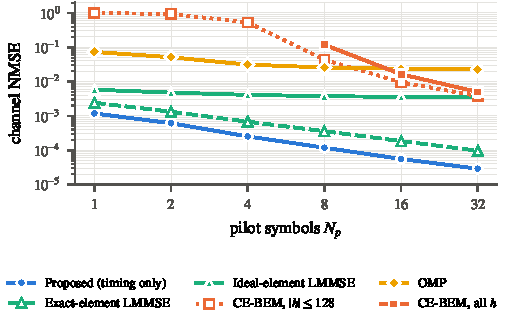
\includegraphics[width=0.62\textwidth]{fig_std_pilots.pdf}\end{center}
Shared path, 20\,dB, 1 to 32 pilot symbols, linear NMSE on a log axis.
\begin{itemize}
\item \textbf{Ours} improves about 3\,dB per doubling of pilots ($-29.3$ to $-45.4$\,dB).
\item \textbf{Exact-element LMMSE} runs parallel, 3--5\,dB worse.
\item \textbf{Ideal-element LMMSE} saturates at $-24.6$\,dB (model-error floor).
\item \textbf{CE-BEM} needs 8 or more pilots to estimate anything; the all-harmonics version is run from 8.
\item \textbf{OMP} saturates near $-16$\,dB.
\end{itemize}
\textbf{Message:} pilot efficiency. Ours is the only estimator within 0.3\,bit/s/Hz with 32 pilots or fewer: 2 on the shared
path, 4 on TDL-C.

\subsection*{$\bigstar$ Fig.~8: coded block error rate}
\begin{center}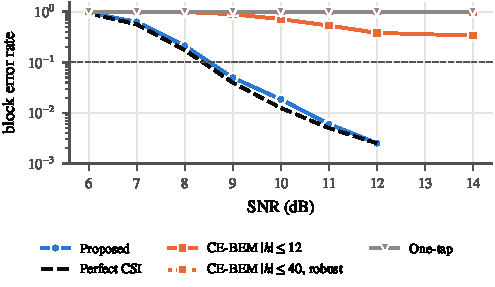
\includegraphics[width=0.55\textwidth]{fig_bler.pdf}\end{center}
\begin{itemize}
\item \textbf{Setup:} rate-1/2 convolutional code, 16-QAM, soft decisions (LLRs) from each receiver's own estimate, 2000
blocks per point, 2 pilots.
\item \textbf{Result:} ours crosses 10\% BLER at 8.51\,dB against 8.37\,dB with perfect CSI, \textbf{a gap of 0.14\,dB
[0.09, 0.20]}. One-tap never decodes; truncated CE-BEM floors at 34\%.
\item \textbf{Message:} the rate metric's conclusion holds on a real coded link.
\end{itemize}

\paragraph{Ranking if asked.} Fig.~6 (proves the mechanism and baseline fairness) $>$ Figs.~4--5 (the standard comparison)
$>$ Fig.~8 (practical proof) $>$ Figs.~2--3 (model and motivation, reproducing Iudice) $>$ Fig.~7 $>$ Fig.~1.

%=====================================================================
\section{The tables}
\begin{itemize}
\item \textbf{Table I, assumptions A1--A6}, each with a justification and a test of its violation:
  \begin{itemize}
  \item \textbf{A1, pattern known:} control information from the network. Ignoring one of two panels collapses the rate
  to 1.15\,bit/s/Hz.
  \item \textbf{A2, generalized CP:} holds for TDL at 30 and 100\,ns; 300\,ns is out of scope.
  \item \textbf{A3, period $T_u$, aligned up to an offset:} the offset is estimated (Algorithm~2).
  \item \textbf{A4, shared paths:} tested with TDL taps from random directions, CDL, 1024 elements and the near field.
  \item \textbf{A5, channel constant over a refresh block:} coherence time 1188 / 119 / 30 symbols at 3 / 30 / 120\,km/h.
  \item \textbf{A6, noise known, no mutual coupling:} a stated limitation.
  \end{itemize}
\item \textbf{Table II, learned-prior baseline:} matched, shifted and self-trained priors against ours (Section~8).
\item \textbf{Table III, robustness.} The estimator runs \emph{unchanged} on data that break its model: time-domain truth;
switching transients; state-dependent output ($\epsilon=0.2$); joint-state coupling; 10\,MHz resonance spread between
elements; beam squint at $Q=256$. Each case is paired with the same channel without the change; every extra loss is
$\le0.05$\,bit/s/Hz.
\item \textbf{Table IV, timing.} BS-locked RIS with offset ignored: 1.62 / 4.23 loss. With Algorithm~2: within 0.011 /
0.033 of known timing. Incident-locked RIS: running the search costs nothing. Sync error up to 150\,ns breaks a fixed window,
not the evidence-chosen one. One pilot: the evidence beats the residual by 1.49 / 2.83.
\item \textbf{Table V, pilot overhead under mobility, held out.} Pilot settings are chosen on 20 channels and reported on
20 different ones. Ours beats the best CE-BEM in all 24 cases, by 1.0--3.9\,bit/s/Hz. Choosing on the reported channels
changes results by at most 0.13. \textbf{Limit:} at 120\,km/h on TDL, ours keeps only 46--66\% of the perfect-CSI rate.
\end{itemize}

%=====================================================================
\section{Repository architecture (what your supervisor will browse)}
{\small
\begin{verbatim}
RIS/
|- Base_Papers/        4 key papers (Iudice 2026, Xu & Petropulu 2023,
|                      Tang 2007 CE-BEM, Mizmizi 2024) - not in git
|- old_ris_project/    earlier unrelated work
`- tm_ris_ofdm/
   |- README.md        chronological lab notebook: Gates 1-3, Weeks 3-12,
   |                   every result including dropped ones
   |- REPRODUCE.md     how to rebuild/rerun every paper item
   |- matlab/          ~100 scripts + core functions (base MATLAB R2026a)
   |- results/         raw per-channel JSON of every run + PREREG_LOG,
   |                   CLAIMS_LEDGER, SUMMARY_*, SOFTENED_CLAIMS
   |- figures/         Python: make_ieee_figures.py, analyse_heldout.py,
   |                   analyse_week12.py, analyse_snr_tang.py, k3_emission.py
   |- paper/ieee/      THE paper: main.tex -> tm_ris_receiver_ieee.pdf
   |                   (11 pages), fig_system.tex, one fig_*.pdf per graph
   |- paper/journal/   extended draft (older; lacks the latest results)
   `- report/          HTML learning guide; this guide
\end{verbatim}}

\paragraph{Core MATLAB functions to name.}
\begin{center}\small
\begin{tabularx}{\textwidth}{lX}
\toprule
File & Role\\
\midrule
\texttt{coupling\_matrix.m}, \texttt{harmonic\_coeffs.m} & ground-truth $\bm H$ (Iudice's equation)\\
\texttt{element\_response.m}, \texttt{params\_openris.m} & the OpenRIS $\Gamma_s(f)$; also \texttt{'ideal'} ($\pm1$) and
\texttt{'state1'/'state2'} indicator modes. The indicator mode is how the kernels $\bm T$ are built without any element model.\\
\texttt{phys\_channel.m} & shared-path channel: LoS plus 5 paths, Rician $K=10$\,dB, 30\,ns rms, geometric element phases\\
\texttt{tdl38901.m}, \texttt{tdl38901\_paths.m} & 3GPP TDL-A/C/D with taps from random directions\\
\texttt{dpss\_basis.m} & DPSS basis and eigenvalues\\
\textbf{\texttt{est\_general.m}} & \textbf{Algorithm 1 (ours)}\\
\texttt{est\_bem\_cg.m} & CE-BEM baseline, matrix-free, equal to the dense solver to $7\cdot10^{-9}$\\
\texttt{fast\_coupling.m} & fast products for CG\\
\texttt{ici\_matrix.m} & Doppler subcarrier mixing for mobility\\
\texttt{fig\_data\_coupling.m} & coupling matrices for Fig.~3\\
\bottomrule
\end{tabularx}
\end{center}
The ideal, exact, mismatched, OMP and learned estimators are local functions inside the scripts that use them, e.g.\
\texttt{week10\_fair\_baselines.m}, \texttt{week12\_standard\_curves.m}, \texttt{week12\_snr\_tang.m}, \texttt{week12\_c6b.m}.

\paragraph{Which script makes which figure.}
\begin{center}\small
\begin{tabularx}{\textwidth}{lXl}
\toprule
Paper item & MATLAB script $\to$ result file & Figure / analysis script\\
\midrule
Fig.~1 & none (TikZ, \texttt{paper/ieee/fig\_system.tex}) & pdflatex\\
Fig.~2 & none (closed form) & \texttt{make\_ieee\_figures.py struct}\\
Fig.~3 & \texttt{fig\_data\_coupling.m} $\to$ \texttt{fig\_coupling\_data.json} & \texttt{make\_ieee\_figures.py struct}\\
Figs.~4--5 & \texttt{week12\_snr\_tang.m} (Step 11: 10:5:40; Step 12: \texttt{snrs=10:2:30}) & \texttt{make\_ieee\_figures.py tang}, \texttt{analyse\_snr\_tang.py}\\
Figs.~6--7 & \texttt{week12\_standard\_curves.m} & \texttt{make\_ieee\_figures.py std}, \texttt{analyse\_week12.py}\\
Fig.~8 & \texttt{week11\_coded\_stats.m} & \texttt{make\_ieee\_figures.py}\\
Table II & \texttt{week12\_c6\_lowsnr.m}, \texttt{week12\_c6b.m} & \texttt{analyse\_week12.py}\\
Table V & \texttt{week11\_overhead\_heldout*.m} & \texttt{analyse\_heldout.py}\\
\bottomrule
\end{tabularx}
\end{center}

\paragraph{Method of work (be proud of this, and know it).}
\begin{itemize}
\item \textbf{Pre-registration:} every test's pass/fail rule is written in \texttt{PREREG\_LOG.md} and committed
\emph{before} the run. Git history proves the order.
\item \textbf{30 channels per point}, paired 95\% $t$-intervals, a clustered bootstrap for error-rate ratios.
\item \textbf{Selection versus reporting:} settings chosen on separate channels and reported on held-out channels.
\item \textbf{Results are never overwritten} (the \texttt{\_loaded} timing run was kept and labelled).
\item \textbf{The claims ledger} gives each claim a status: OK, FIXED, NARROWED, WITHDRAWN or FAIL.
\end{itemize}

\paragraph{Project history.}
(1) Gate~1: reproduce Iudice's model. (2) Gate~2: equalization. (3) Gate~3: estimation; the first attempt failed, the
physics-aware second passed. (4) Weeks 3--8: extensions, hardware, timing, baselines, mobility. (5) Weeks 9--11: external
review workstreams (fairness, held-out tests, timing physics, equalizer timing). (6) Week~12: standard curves, the learned
baseline, distribution shift, and the base-paper-format figures (Steps 11--12, SNR 10--40 and 10--30\,dB).

%=====================================================================
\section{Negative results and limits (say them before he finds them)}
\begin{enumerate}
\item \textbf{A learned prior beats ours on matched channels.} An LMMSE whose prior is learned from 100 or more channels of
the same distribution is better: 0.006 vs 0.070 at 20\,dB on the shared path, 0.074 vs 0.285 on TDL-C.
  \begin{itemize}
  \item \textbf{Reason:} our simulated families are low-dimensional. 1000 shared-path channels span 6 principal components
  with mean correlation 0.92 (narrow 7.7\,MHz band, strong line of sight); TDL has fixed tap delays ($\approx$50 components).
  \item \textbf{Under distribution shift} (trained 30\,ns $\to$ tested 100\,ns) it is worse than ours by 0.22 / 0.95 at 20 /
  30\,dB; TDL-C$\to$D: tie / ours better by 0.37; TDL-C$\to$A: learned still better by 0.06.
  \item \textbf{The self-trained prior} (learned from our own 8-pilot estimates, no true channels, no element model) beats
  plain ours by 0.042 / 0.107. Adopted as an optional second stage.
  \item \textbf{Claim changed} from ``beats every baseline'' to \textbf{``best among estimators needing no training data''}.
  \end{itemize}
\item \textbf{Low SNR:} receivers given the element model are slightly better than ours at low SNR ($\le0.03$ shared,
$\le0.06$ TDL-C); the crossover is between 17 and 22\,dB depending on the channel set. A pre-registered SNR-adaptive rank fix
\textbf{failed} (worse by 0.034 at 20\,dB on TDL-C), so the frozen rank stays.
\item \textbf{High SNR on rich multipath:} on TDL-C above $\sim$33\,dB, CE-BEM with 8$\times$ our pilots reaches lower BER
(model-error floor; Section~5).
\item \textbf{Mobility:} at 120\,km/h on TDL, ours keeps only 46--66\% of the perfect-CSI rate. A limit of pilot-based
estimation, not of the model.
\item \textbf{300\,ns delay spread:} the CP condition fails (A2), so it is out of scope. A two-timescale attempt was withdrawn.
\item \textbf{Equalizer speed:} ``2.6$\times$ faster'' was withdrawn. CG is faster only up to about 12 symbols per estimate.
\item \textbf{Simulation only:} one published cell, no mutual coupling, no over-the-air test.
\item \textbf{Time modulation costs rate.} A static RIS optimized for the user gives 6.66\,bit/s/Hz against 2.98--5.35 for a
TM-RIS with our receiver. TM is for security, harmonic steering or sensing, not single-user rate. An eavesdropper with
generic CE-BEM still gets 1.8--2.2\,bit/s/Hz, so the pattern must be kept secret.
\item \textbf{Statistics:} many comparisons without a multiple-comparison correction. Effect sizes are mostly large relative
to the intervals, but say so if asked.
\item \textbf{One pre-registered sanity check failed:} truncated CE-BEM loses rate from 20 to 30\,dB even with the oracle
robust equalizer (its error sits on the missing harmonics). Reported, not hidden.
\end{enumerate}

%=====================================================================
\section{Delay spread versus coherence time (the ``300 ns'' question)}
In this project 300\,ns is the \textbf{RMS delay spread} of the 3GPP TDL models (scaled to 30, 100 or 300\,ns), \textbf{not}
the coherence time.
\begin{center}\small
\begin{tabular}{lll}
\toprule
 & Delay spread & Coherence time\\
\midrule
Caused by & multipath: echoes at different delays & motion: Doppler shift\\
Describes & how the channel changes \textbf{across frequency} & how the channel changes \textbf{over time}\\
Set by & the scattering environment & speed and carrier frequency\\
In our runs & 30 / 100 / 300\,ns & 3 / 30 / 120\,km/h\\
\bottomrule
\end{tabular}
\end{center}
\textbf{Frequency side.} Coherence bandwidth $\approx 1/(5\times$ delay spread$)$: 30\,ns $\to$ 6.7\,MHz; 100\,ns $\to$
2\,MHz; 300\,ns $\to$ 0.67\,MHz. At 300\,ns the channel changes noticeably every few hundred kHz across the 100\,MHz band,
giving the low-rank model more unknowns, and the CP condition fails. Hence the open limitation.

\textbf{Time side.} At 3.594\,GHz, $f_D=vf_c/c$ and coherence time $\approx0.423/f_D$:
\begin{center}\small
\begin{tabular}{lll}
\toprule
Speed & Doppler shift & Coherence time\\
\midrule
3\,km/h & $\sim$10\,Hz & $\sim$42\,ms\\
30\,km/h & $\sim$100\,Hz & $\sim$4.2\,ms\\
120\,km/h & $\sim$400\,Hz & $\sim$1\,ms\\
\bottomrule
\end{tabular}
\end{center}
These are the numbers behind the pilot-overhead table: faster users need pilots more often. Older (non-paper) figures:
\texttt{figures/fig14\_tdl\_channels.png} (delay spread: gap vs pilots for TDL at 100 and 300\,ns) and
\texttt{figures/fig11\_mobility.png} (gap vs symbols since the pilots at 3/30/120\,km/h). In the paper these results are in
the robustness and overhead tables.

%=====================================================================
\section{Numbers to have in your head}
\begin{center}\small
\begin{tabularx}{\textwidth}{lX}
\toprule
Item & Value\\
\midrule
Setup & n78, $f_c$ 3.594\,GHz, $\Delta f$ 30\,kHz, CP 2.34\,$\mu$s, $Q=16$ ($4\times4$, $\lambda/2$), $K=8$, $D=0.75$\\
Comparison size & $M=256$ (7.7\,MHz), central 128 subcarriers scored (avoids band-edge truncation of harmonics)\\
Full band & $M=3276$ (98\,MHz)\\
Estimator settings & shared path $\tau_{\max}$ 0.3\,$\mu$s, $L=16$, $r=8$; TDL $\tau_{\max}$ 1\,$\mu$s, $L=\lceil M\Delta f\tau\rceil+10$, $r=16$\\
Element (in channel) & phase drift 46.4$^\circ$/49.1$^\circ$; difference $180^\circ\pm7.8^\circ$; imbalance 0.57\,dB; loss 1.01\,dB\\
One-tap ceiling & $-4.8$\,dB SIR\\
Harmonic tail & 3.4 / 1.0 / 0.32\% at $H=12$ / 40 / 128; floor $-14.7$\,dB\\
Unknowns & $3Lr+Gr^2=448$ vs $M^2=65{,}536$\\
Pilots needed ($\le0.3$ loss) & 2 (shared), 4 (TDL-C); all classical baselines $>32$\\
SNR curves (Fig.~4) & ours NMSE $-23.7\to-41.3$\,dB, loss 0.035--0.121 over 10--30\,dB\\
Crossover vs genie & 17--22\,dB depending on channel set\\
Paired gain over best model-based baseline & 0.41 / 2.16 (shared, $N_p=2$, 20 / 30\,dB)\\
Coded gap & 0.14\,dB [0.09, 0.20]\\
Full-band SER ratio vs perfect & 1.10 (16-QAM, 20\,dB), 1.37 (64-QAM, 28\,dB)\\
CG & tolerance $3\cdot10^{-3}$, 8--20 iterations, break-even $\approx$12 symbols\\
Hardware limits & CFO $<1$\% of spacing, phase noise $<100$\,Hz linewidth, jitter $<4$\,ns rms (30\,dB), rise time $\le42$\,ns needs no calibration\\
Emission (ACLR) & 36.8\,dB with ideal edges (BS limit 45\,dB), 52.7\,dB with 0.05-slot edges\\
\bottomrule
\end{tabularx}
\end{center}

%=====================================================================
\section{Questions your supervisor is likely to ask, with answers}

\subsection{Fundamentals and the model}
\Q{Why does time modulation break OFDM's diagonal channel?}
The switching is periodic in time, i.e.\ multiplication by a periodic waveform. In frequency that is convolution with a
Fourier series, so subcarrier $m$ leaks into $m+h$ with weight $b^{[h]}$. The CP removes inter-symbol interference but
cannot undo a channel that changes inside the symbol.
\Q{Why is the switching period $T_u$ and not $T_u+T_{cp}$?}
That is the Iudice model with the pattern synchronized to the useful symbol (A3; TM-IRS designs do this). The CP part is
discarded at the receiver. A misalignment is exactly the offset $d$ that Algorithm~2 estimates.
\Q{What exactly is the generalized CP condition?}
The CP must cover the cascaded channel delay spread plus the element memory (13.8\,ns). Under it there is no ISI and no
channel-induced ICI; only the structured RIS coupling remains. Checked numerically: $\le-56$\,dB of energy beyond the CP for
TDL at 30 and 100\,ns, violated at 300\,ns.
\Q{Is $\bm H$ Toeplitz?}
No. The kernels $\bm T_{q,s}$ are Toeplitz, but $\bm v_{q,s}=\bm\Gamma_s\odot\bm a^{\rm s}$ depends on the input frequency,
so $\bm H=\sum\bm T\circ(\bm a\bm v^{\T})$ is not. For ideal flat elements and flat channels it would be. That is why
Toeplitz-based eavesdropper methods (Tao et al.) do not carry over.
\Q{Derive the one-tap SIR bound.}
The DC coefficient is $2D-1$ and the total energy is 1 by Parseval, so the one-tap receiver collects $(2D-1)^2$ and the rest
is interference: $0.25/0.75\Rightarrow-4.8$\,dB at $D=0.75$.
\Q{Why $1/H$ decay of the harmonic tail?}
A step edge gives $|t[h]|\lesssim|\mathrm{sinc}(h/K)|\sim1/h$, so energy decays as $1/h^2$ and the energy beyond $H$ as
$\sum1/h^2\sim1/H$. Finite rise times make it decay faster (an extra sinc factor).
\Q{Where does the element model enter, and why don't you need it?}
Only through $\bm v=\bm\Gamma\odot\bm a^{\rm s}$, multiplied by the unknown BS--RIS channel. Since $\bm a^{\rm s}$ must be
estimated anyway, estimating the product costs nothing extra (Cor.~1).
\Q{Is your evaluation circular?}
The ground truth (Iudice's model) is exact for Prop.~1, but the estimator adds structure the truth does not have: low rank
and the DPSS prior. Table~III tests the estimator on data from outside its model: time-domain simulation, transients,
state-dependent output, coupling between states, element spread and squint. What remains untested is the single-resonance
element and mutual coupling, which needs over-the-air or full-wave validation.
\Q{Mutual coupling between elements?}
Ignored, as in Iudice; a stated limitation. It would make the element response depend on the neighbours' states, breaking
the per-element separation. Table~III's ``joint-state coupling, $\kappa=0.08$'' is a proxy test, costing $\le0.015$\,bit/s/Hz.
\Q{What about the direct BS--user path?}
It is the special case where $\bm v$ is the same in both states; since $\bm T_1+\bm T_2=\bm I$ the model contains it
unchanged. Tested: 5.28 / 8.13 against 5.39 / 8.49\,bit/s/Hz with perfect CSI.

\subsection{The estimator}
\Q{Why DPSS?}
They are the orthonormal basis with maximal energy concentration for responses limited to a delay window: the eigenvectors
of the sinc correlation (Slepian). The eigenvalues give a natural prior, so about $M\Delta f\tau_{\max}+1$ coefficients carry
the energy.
\Q{Why LMMSE / Bayesian rather than least squares?}
448 unknowns against 512 noisy observations: least squares is ill-conditioned. The prior regularizes it in a principled
way, and the square-root form stays stable when prior variances are tiny.
\Q{Is ALS guaranteed to converge to the global optimum?}
No, it is non-convex. Each block update is an LMMSE, so the objective decreases monotonically, but with no global
guarantee. The linear-LMMSE initialization lands it in 1--2 iterations; random starts are 3--5$\times$ worse.
\Q{Identifiability and ambiguities?}
$\bm U\bm\Lambda\bm V^{\T}$ has a gauge ambiguity ($\bm U\to\bm U\bm A$, $\bm\Lambda\to\bm A^{-1}\bm\Lambda\bm B^{-\T}$,
$\bm V\to\bm V\bm B$), but $\bm H$ is unaffected; only the product matters, and $\bm H$ is what we evaluate.
\Q{How did you choose the rank $r$?}
Frozen before the tests: 8 for the shared path, 16 for TDL. An ablation (\texttt{week10\_ablation}) shows $r=2$--8 similar
on the shared path, while TDL needs more. The SNR-adaptive rank was tested and failed its pre-registration.
\Q{How close are you to the Cram\'er--Rao / Bayesian bound?}
For the linear stage, 5--6\,dB above the Bayesian bound under the assumed prior ($-26.4$ vs $-32.4$\,dB at 20\,dB, 2 pilots).
The gap comes from prior mismatch: real delays are not uniform in the window. A full CRB for the nonlinear low-rank model
was not derived. That is an honest gap.
\Q{Non-identical patterns per element?}
Handled by $G$ groups with $\bm\Lambda_g$. With 16 distinct random patterns, 4 pilots are needed (numbers in the README).
\Q{Why does ours beat the exact-element LMMSE?}
That LMMSE is linear with a full $L\times L$ coefficient matrix (256 unknowns). Ours imposes rank $r$, so it removes more
noise. At low SNR the nonlinear fit costs a little, which explains the crossover at 17--22\,dB.

\subsection{Timing}
\Q{Why can't you just pick the offset by the smallest pilot residual?}
By Prop.~2 a wrong offset is equivalent to delaying one hop and advancing the other. The basis can absorb small shifts
(residual only $2.7\cdot10^{-4}$ at 100\,ns), so the residual is flat. The evidence's log-det term penalizes the improbable
shifted responses. Residual search works with 2 or more pilots on a fine grid, but overfits with 1 pilot and is 5--58$\times$
slower.
\Q{What is the physical size of the offset?}
Zero if the RIS locks to the incident signal; $-\tau_b$ (its distance to the BS, 50--300\,ns) if it locks to the BS clock
(Prop.~3).
\Q{Why must the window start $t_0$ be estimated too?}
After synchronization the first arrivals of the two hops sum to zero, up to the offset. A window starting late cannot hold
both hops. A sync error of $\pm150$\,ns breaks a fixed window (0.22 / 1.16 loss), but not the evidence-chosen one.
\Q{What about random jitter on the switching edges?}
It cannot be estimated. It must stay below about 4\,ns rms at 30\,dB (20\,ns at 20\,dB); ordinary clocks have picosecond
jitter.

\subsection{Equalizer and complexity}
\Q{Why CG instead of a direct solve?}
Memory and products: $\bm H\bm x$ costs $O(rM\log M)$ without forming $\bm H$. A dense solve needs 172\,MB at $M=3276$ and
687\,MB at 6552.
\Q{Then why is dense faster for slow channels?}
The factorization happens once per estimate and runs as level-3 BLAS; each symbol then costs $O(M^2)$, cheap in practice.
Measured break-even about 12 symbols, not the 140 from operation counts; the old 2.6$\times$ claim was withdrawn.
\Q{How was the CG tolerance chosen?}
By a pre-registered sweep: $3\cdot10^{-3}$ is within 2\% of the dense error rate at every $M$; $10^{-2}$ is 15\% worse at
$M=3276$.
\Q{How is warm-starting used?}
A refresh starts from the previous factors (two ALS iterations, no linear stage): 1.4\,s against 12.5\,s from scratch, with
the same SER.

\subsection{Evaluation methodology}
\Q{Why that rate metric?}
The MMSE filter is built from the estimate and applied to the \textbf{true} channel. Residual interference is treated as
Gaussian noise, giving an achievable-rate proxy under mismatched channel knowledge. The coded BLER (Fig.~8) confirms it.
\Q{What is ``robust MMSE''?}
The MMSE with the estimation-error power added to $\sigma^2$. Every estimator got three equalizers (naive, residual-based
robust, oracle robust); paired comparisons take each baseline's best.
\Q{Why $M=256$ and only the central 128 subcarriers?}
Baselines need dense $M\times M$ matrices, so cost forces $M=256$. Harmonics leak beyond the band edges and are truncated
there, so scoring the central half avoids edge artefacts. The full band ($M=3276$) is validated separately: SER, coded link,
timing.
\Q{Is 30 channels enough, and what about multiple comparisons?}
Paired designs reduce variance, and the intervals are reported. There is no multiple-comparison correction; the main effects
are many times the interval width. Be honest here.
\Q{What does pre-registration buy you?}
Rules are fixed before results exist, failures are reported, and git timestamps prove the order.
\Q{Selection bias in the overhead table?}
Pilot settings were chosen on 20 channels and reported on 20 others. In-sample selection changes results by at most 0.13.

\subsection{Baselines and fairness}
\Q{Were the baselines given a fair chance?}
CE-BEM was allowed up to all $2M-1$ harmonics and up to 32 pilots, solved matrix-free and checked against the dense solver.
All estimators got the same three equalizers. The ideal-element LMMSE uses our own prior. A pre-registered sanity check that
failed was reported, not hidden.
\Q{Isn't the ideal-element baseline a straw man?}
Fig.~6: with ideal elements it equals ours, so it fails only because of the element assumption.
\Q{Why no neural-network baseline?}
The learned-prior LMMSE is the Bayes-optimal linear estimator for the learned statistics, which a squared-error-trained
network approaches for near-Gaussian channels. Base MATLAB has no deep-learning toolbox. It beats ours on matched channels
and loses under shift (Table~II).
\Q{If a learned prior beats you, why use yours?}
(1) Ours needs \textbf{no training data and no element model}. (2) Offline priors break under a change in delay spread or
line-of-sight strength. (3) Ours can \textbf{generate its own training data}, and the self-trained prior keeps most of the
gain. (4) Real deployments are richer than our low-dimensional simulated families.

\subsection{Practicality and system level}
\Q{Is assumption A1 (pattern known) realistic?}
Yes, the network configures the RIS; it is control-plane information like a pilot configuration. In a security scenario
the pattern must be secret from the eavesdropper, which is why the eavesdropper result matters.
\Q{Then why use a TM-RIS at all, given a static RIS gives more rate?}
A TM-RIS is for physical-layer security, harmonic beam steering or sensing. Our point is that the legitimate user does not
have to lose the coupled energy.
\Q{Mobility?}
Doppler mixing within a symbol is $-60$ / $-47$ / $-34$\,dB at 3 / 30 / 120\,km/h, so ageing of the estimate dominates.
Pilots are re-sent with selected spacing. Decision-directed trackers were worse because errors accumulate.
\Q{Hardware impairments?}
CFO under 1\%, phase noise under 100\,Hz or tracked, rise times up to 42\,ns fine (longer ones calibrated or fitted
blindly), emission 36.8\,dB ACLR with ideal edges against the BS limit of 45\,dB. A passive RIS has no requirement of its
own, but smoother edges (0.05 slot) give 52.7\,dB.
\Q{Scaling with a larger RIS?}
The low rank is set by the number of paths, not $Q$. Effective rank 5 / 9 / 13 / 16 for $Q=16$ / 64 / 256 / 1024 (CDL-C,
98\,MHz, with squint).
\Q{Multi-user, MIMO base station, uplink?}
Not done. The separation holds for each link, but multi-user pilot design and MIMO are future work.

\subsection{Novelty and literature}
\Q{What is new compared with Iudice 2026?}
They model the channel and assume it known, and name equalization as future work (their Sec.~V). We give the estimator,
the blind timing, the equalizer and the evaluation.
\Q{Compared with Xu \& Petropulu, and Tao et al.?}
They assume ideal flat $\pm1$ elements and a one-tap receiver for the legitimate user. Tao's eavesdropper relies on Toeplitz
structure, which dispersive elements break.
\Q{What do you adopt rather than claim?}
The DPSS basis (Slepian, Zemen), low-rank RIS models, matrix-free CG (Hrycak), Bayesian evidence (MacKay), the CE-BEM
baseline and its figure format (Tang).
\Q{What would you do next?}
An over-the-air or full-wave test with mutual coupling; the 300\,ns regime (a longer CP, or a two-timescale model done
properly); a multi-user / MIMO extension; a Cram\'er--Rao bound for the low-rank model; testing more pilots or a higher rank
on TDL-C at high SNR.

\subsection{The figures (new questions from the latest changes)}
\Q{Fig.~6: so your model only works for ideal cases and not for real ones?}
No, the opposite. The literature's ideal-element estimator works only at $\alpha=0$; ours is flat for every $\alpha$
because it never assumes an element model. See Section~5.
\Q{Your model is good only up to about 25\,dB?}
No. On the shared path it is best at every SNR up to 40\,dB (loss 0.26 at 40\,dB). On TDL-C its loss to perfect CSI grows
above $\sim$22\,dB because of a model-error floor that every estimator has, but it keeps the lowest NMSE and rate loss up to
40\,dB; only CE-BEM with 8$\times$ our pilots gets a lower BER, from about 33\,dB.
\Q{Why do Figs.~4--5 stop at 30\,dB when Tang go to 40\,dB?}
Practical links mostly run at 0--30\,dB, and the graphs are computed on a 2\,dB grid over exactly that range. The 35--40\,dB
results (same run, 5\,dB grid) are stated in the text, including the one where CE-BEM wins.
\Q{Why does the exact-element genie beat you below about 20\,dB?}
It is a linear LMMSE handed the true element model, so it needs no nonlinear fit; when noise dominates, that matters more
than our smaller number of unknowns. It is a reference, not a practical receiver.
\Q{Why does your element figure not match Iudice's exactly?}
Iudice's curves are full-wave; ours use their fitted single-pole model with their Table~I parameters. Differences are about
a degree and a fraction of a dB (Section~5).
\Q{What is the checkerboard in Fig.~3(a)?}
With $K=2$ the switching is a square wave with 50\% duty, whose even Fourier coefficients vanish, so every second
off-diagonal is zero.

\subsection{Repository and reproducibility}
\Q{How do I reproduce Figs.~4--5?}
Run \texttt{matlab/week12\_snr\_tang.m} with \texttt{parts=1; snrs=10:2:30; icsel=1} (and \texttt{icsel=2}),
$\sim$3\,h with the two in parallel, writing \texttt{results/week12\_snr\_tang\_fine\_*.json}; then
\texttt{figures/make\_ieee\_figures.py tang}. Same seeds give identical numbers (the 10/20/30\,dB values equal the 5\,dB-grid
run exactly). For a smoke test set \texttt{ntrial = 1} and a different \texttt{outname}.
\Q{What is \texttt{week11\_eq\_amortised\_loaded.json}?}
The first timing run, which overlapped another job. It was kept and labelled, not used for timing claims, and that deviation
is logged in the pre-registration log.
\Q{Why are there withdrawn results in the README?}
The README is the lab notebook. \texttt{SOFTENED\_CLAIMS.md} and the claims ledger list what changed and why. Nothing was
deleted.

%=====================================================================
\section{Three sentences to open with if he says ``summarize your work''}
\begin{keybox}
\begin{enumerate}
\item \emph{``Time-modulated RIS couples OFDM subcarriers, and with real, non-ideal elements nobody had a receiver for it.
Iudice et al.\ left equalization as future work.''}
\item \emph{``I showed that the coupling separates exactly into timing kernels the receiver knows and a low-rank propagation
part that absorbs the element response, so the receiver needs no element model. On that I built an estimator that works
from 2--4 pilots, a blind clock-offset estimator based on the offset being an opposite delay, and a matrix-free
equalizer.''}
\item \emph{``In pre-registered tests it beats every estimator needing no training data and decodes within 0.14\,dB of
perfect channel knowledge. I also report where it loses: a learned prior on matched channels, low SNR, very high SNR on rich
multipath, 120\,km/h, and 300\,ns.''}
\end{enumerate}
\end{keybox}

\end{document}
